\begin{corollary}[The explicit power gap of version 1]
\label{cor:v1-power-gap}
Fix \(0<\eta<3/4\), and let \(H\) be the largest dyadic integer
at most \(N^{1/4}\). For sufficiently large \(N\),
\[
 H\le N^{1-\eta},\qquad
 \E_{\mathbf1}(N,H)\ge\frac1{16}N^{9/4},\qquad
 \frac{N^{2+1/8}}H\le2N^{15/8}.
\]
Consequently no constant independent of the bounded coefficient
sequence and of \(N\) can make the proposed collar bound hold
at \(\varepsilon=1/8\). The ratio of the displayed lower bound
to the proposed scale grows at least as \(N^{3/8}/32\).
\end{corollary}
\begin{proof}
The choice gives \(N^{1/4}/2<H\le N^{1/4}\). The condition on
\(\eta\) places this block in the stated range. For large \(N\),
\(2H\le N/2\); hence Proposition~\ref{prop:uniform} gives
\(\E_{\mathbf1}(N,H)\ge HN^2/4>N^{9/4}/8\).
We weaken the constant to retain the original displayed bound.
Also \(N^{17/8}/H<2N^{17/8-1/4}=2N^{15/8}\).
Subtracting the exponents gives \(9/4-15/8=3/8\).
\end{proof}

\begin{figure}[ht]
\centering
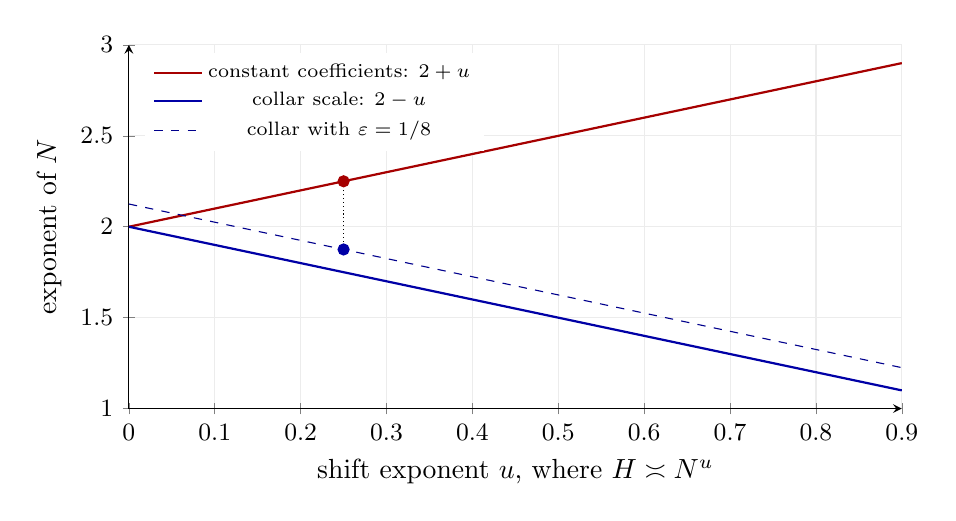
\begin{tikzpicture}
\begin{axis}[width=.94\linewidth,height=6.2cm,
 xmin=0,xmax=.9,ymin=1,ymax=3,
 xlabel={shift exponent \(u\), where \(H\asymp N^u\)},
 ylabel={exponent of \(N\)},grid=major,grid style={gray!15},
 axis lines=left,tick label style={font=\small},
 legend style={at={(.02,.98)},anchor=north west,draw=none,font=\scriptsize}]
\addplot[red!65!black,thick,domain=0:.9,samples=2]{2+x};
\addlegendentry{constant coefficients: \(2+u\)}
\addplot[blue!65!black,thick,domain=0:.9,samples=2]{2-x};
\addlegendentry{collar scale: \(2-u\)}
\addplot[blue!55!black,dashed,domain=0:.9,samples=2]{2.125-x};
\addlegendentry{collar with \(\varepsilon=1/8\)}
\addplot[only marks,mark=*,red!65!black] coordinates {(.25,2.25)};
\addplot[only marks,mark=*,blue!65!black] coordinates {(.25,1.875)};
\draw[densely dotted] (axis cs:.25,1.875)--(axis cs:.25,2.25);
\end{axis}
\end{tikzpicture}
\caption{The original exponent-gap comparison, with the
\(\varepsilon=1/8\) line made explicit. At \(u=1/4\) the marked
exponents are \(9/4\) and \(15/8\). For each fixed \(0<u<1\),
the exact maximum has exponent \(2+u\). The point \(u=1\) is
excluded: the block \(H=N\) contains no admissible shifts.}
\label{fig:v1-gap}
\end{figure}

\begin{lemma}[Square divisors and the signed correlation]
\label{lem:v1-square-divisor}
For every positive integer \(n\),
\[
 \lambda(n)=\sum_{r^2\mid n}\mu(n/r^2).
\]
Consequently, for integers \(Y\ge1\) and \(h\ge1\),
\begin{equation}\label{eq:v1-square-correlation}
 C_{\lambda,h}(Y)=
 \sum_{r\le\sqrt Y}\ \sum_{s\le\sqrt{Y+h}}
 \ \sum_{\substack{1\le n\le Y\\r^2\mid n,\ s^2\mid n+h}}
     \mu(n/r^2)\mu((n+h)/s^2).
\end{equation}
The inner sum is empty unless \(\gcd(r,s)^2\mid h\).
The summand indexed by \(r=s=1\) is exactly
\(\sum_{n\le Y}\mu(n)\mu(n+h)\).
\end{lemma}
\begin{proof}
Both sides of the first identity are multiplicative. At \(p^e\),
only \(e-2j=0\) or \(1\) contributes to
\(\sum_{2j\le e}\mu(p^{e-2j})\), giving \((-1)^e\).
Insert the identity into each factor of the correlation. All
sums are finite, so rearrangement is exact. The two congruences
\(n\equiv0\pmod{r^2}\), \(n\equiv-h\pmod{s^2}\) are compatible
exactly when \(\gcd(r^2,s^2)\mid h\), by the generalized Chinese
remainder theorem. This gcd is \(\gcd(r,s)^2\). The final
assertion follows by selecting \(r=s=1\).
\end{proof}

This identity preserves the multiplicative signs. The
\(r=s=1\) contribution is one stratum of the exact sum; it
does not approximate the whole correlation without an estimate
for the other strata. Replacing each M\"obius coefficient by its
absolute value would instead return to the coefficient-uniform
obstruction just proved.
